\fancychapter{Implementation}

\section{System Architecture}
This section presents the architecture of the implemented evaluation framework, designed to understand the ability of language models to verify distributed algorithms under different system assumptions. This framework combines a repository of distributed algorithms, a set of prompt templates based on different prompt engineering strategies, and a model interface responsible for querying the selected models with all combinations of algorithms and prompts. The generated outputs are then analyzed and compared according to the correctness properties expected for each algorithm.

The architecture is designed to test the same set of algorithms across different models and prompt types in a consistent way. Each algorithm is paired with each prompt template to create a final model query, which is submitted to each selected model, and each corresponding output is stored for later evaluation. This structure enables us to compare not only the performance of different language models and the knowledge and reasoning across different algorithms but also the impact of prompt engineering on distributed algorithm verification.

The framework is composed of four main components: \textit{the algorithm repository}, \textit{the prompt template repository}, \textit{the model interface}, and \textit{the response storage} and two execution scripts, one for the model interface and another for results storaging.

\begin{figure}[H]
    \centering
    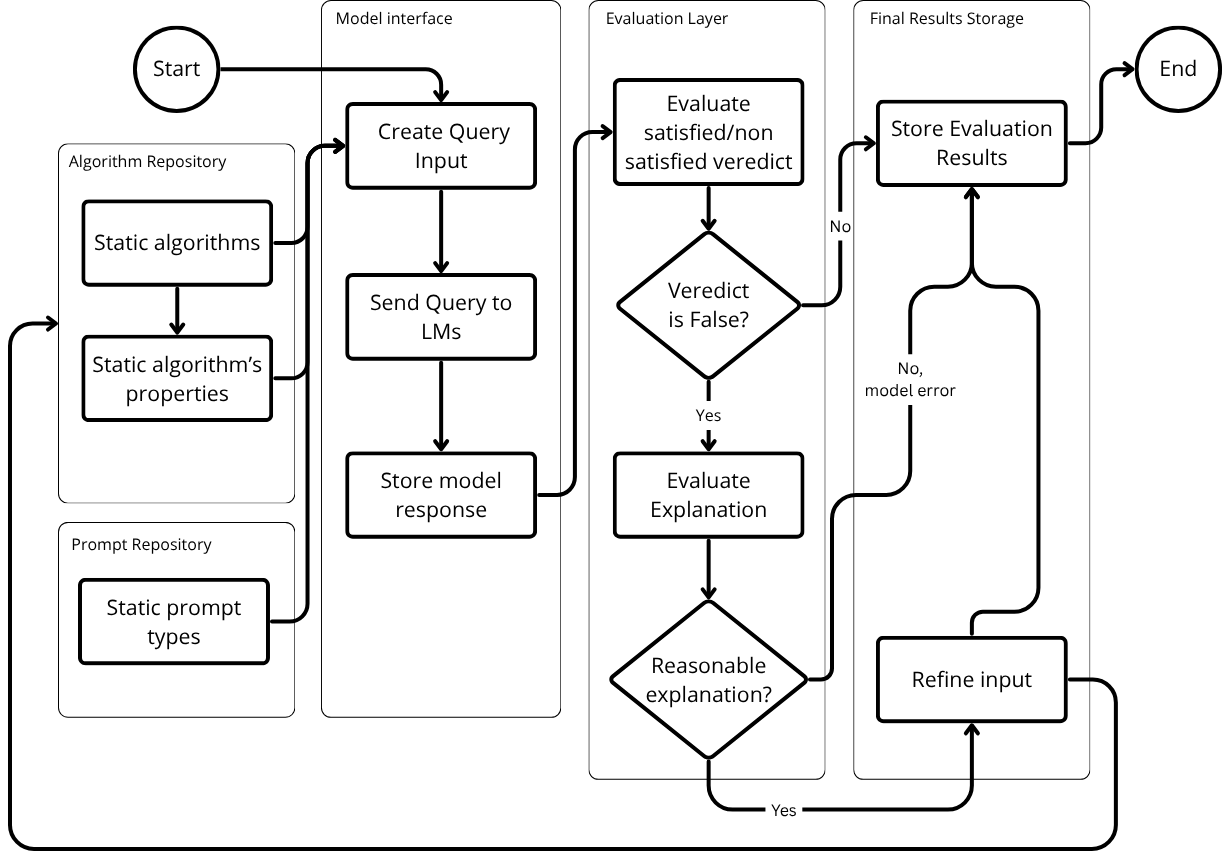
\includegraphics[width=\textwidth]{Images/process-flow.png}
    \caption{Data flow of the evaluation framework.}
    \label{fig:system-data-flow}
\end{figure}

Figure~\ref{fig:system-data-flow} presents the data flow of the evaluation framework. The first elements of the system are the algorithm repository, \texttt{algorithms/} directory, which stores the distributed algorithms used in the evaluation, the \texttt{properties/} directory which stores only the correctness properties to be verified for each algorithm, kept in a separate directory to make them explicit in the prompt input, instead of requiring the model to extract them from the algorithm description itself, and the \texttt{prompts/} directory stores the static prompt templates used in the experiments, containing different prompt formulations, each following a specific prompt engineering strategy. The prompt templates are later combined with the algorithms to create the final prompts submitted to the models, being the model interface responsible for this using a python script that generates all combinations of the set algorithms and their corresponding properties and prompt types, starting the data flow when triggered. This design ensures that all models are evaluated under the same conditions and that differences in the outputs can be attributed to the model or prompt strategy rather than to inconsistencies in the input construction. Each generated prompt is then submitted to each selected model through the model interface. Therefore, the execution covers all combinations of algorithms, prompt strategies, and models. 

Each response is then saved in the \texttt{results/} directory, following a structure organized by algorithm and prompt type. For example, each iteration of the experiment has its results folder, being differenciated with the number of iteration. Inside an interation results folder, each algorithm has its own folder, and inside it the responses are grouped according to the prompt strategy used, and inside the prompt folder there is a file with the result, being its name the model used for this prompt combination. This leads to a very large number of output files due do the density of the experiment. 

The second script is responsible for processing the stored model responses and rebuilding the Excel results file. This script scans all result folders, and treats the folder suffix as the version identifier. Storing the responses separately makes it possible to inspect each result manually when needed, repeat parts of the evaluation, and compare outputs across models and prompt types without rerunning the entire experiment. For each algorithm, it reads the corresponding file in the \texttt{properties/} directory to obtain the list of correctness properties that must be verified, this separation is important because the expected properties are not taken from the model output, they are explicitly defined before evaluation. 

For each stored response, the script parses the model answer and compares it with the expected properties, supporting both plain text responses and JSON-stream responses produced by some model interfaces. Empty files, rate-limit errors, timeouts, connection errors, and unusable JSON-stream responses are classified as execution errors, and responses that do not mention enough expected properties, use wrong property names, or do not follow a recognizable verdict format are classified as incorrect output format. When the response follows the expected structure, the script checks each property individually. A property is counted as satisfied when the answer contains a recognized positive verdict, such as \texttt{[satisfied]}, \texttt{satisfied}, \texttt{true}, or \texttt{yes} and is counted as non-satisfied when the answer contains a recognized negative verdict, such as \texttt{[non satisfied]}, \texttt{not satisfied}, \texttt{false}, \texttt{violated}, or \texttt{not met}. If all expected properties are marked as satisfied, the result is classified as correct, on the other hand, if the response is structured but at least one property is marked as non-satisfied, the result is classified as wrong and the results are written into an Excel workbook. For each experimental version, it creates a separate sheet containing the results organized by algorithm, prompt type, and model, using a color-coded layout: green for correct answers, red for structured but wrong answers, orange for incorrect output format, and gray for execution errors. In addition, the script creates a global comparison sheet that aggregates results across all versions, including success rates by version, model rankings, prompt rankings, algorithm difficulty rankings, heatmaps for model--prompt, model--algorithm, and prompt--algorithm combinations, as well as trend analyses across versions.

This automated processing step is essential because manually inspecting every output file would not be feasible as the number of models, prompts, algorithms, and versions increases. The Excel file centralizes the evaluation results and makes it possible to identify weak prompts, low-performing models, algorithms that are harder to verify, and improvements or regressions between iterations, being easier to, based on the collected results, new iterations of the experiment can be performed while keeping the general evaluation structure consistent.

\begin{table}[H]
\centering
\renewcommand{\arraystretch}{1.25}
\caption{Implementation structure of the evaluation framework}
\label{tab:implementation-structure}
\begin{tabular}{|>{\raggedright\arraybackslash}p{4cm}|
                >{\raggedright\arraybackslash}p{4cm}|
                >{\raggedright\arraybackslash}p{5.5cm}|}
\hline
\textbf{Part of the framework} & \textbf{Project artifact} & \textbf{Role in the experiment} \\
\hline
Algorithm inputs & \texttt{algorithms/} & Stores the normalized algorithm descriptions. \\
\hline
Property inputs & \texttt{properties/} & Stores the properties that each model must verify. \\
\hline
Prompt inputs & \texttt{prompts/} & Stores the static prompt templates. \\
\hline
Experiment runner & Model execution python script & Reads algorithms, properties, and prompts; sends queries to models. \\
\hline
Raw outputs & \texttt{results/} & Stores model responses by algorithm, prompt type, and model. \\
\hline
Results parser & Results analysis pyhton script & Reads output files and classifies each response. \\
\hline
Final analysis & Excel results file & Stores scores, rankings, heatmaps, and comparisons. \\
\hline
\end{tabular}
\end{table}

\subsection{Algorithm and Prompt Repositories Component}
\subsubsection{Problem Selection}
The evaluation focuses on broadcast distributed algorithms, selected because they represent core communication abstractions in distributed systems while still allowing the verification task to be controlled and comparable across models. Each algorithm is represented with its corresponding system assumptions, fault model, and correctness properties as well as other algorithm's related information. In order to avoid bias caused by differences in presentation, all algorithms were rewritten using the same structured template as represented in ~\ref{tab:algorithm-template-structure}:

\begin{table}[H]
\centering
\renewcommand{\arraystretch}{1.25}
\caption{Structure of the algorithm input template}
\label{tab:algorithm-template-structure}
\begin{tabular}{|>{\raggedright\arraybackslash}p{4.2cm}|
                >{\raggedright\arraybackslash}p{9cm}|}
\hline
\textbf{Template field} & \textbf{Purpose} \\
\hline
Identification & Specifies the algorithm name, problem type, fault model, and timing model. \\
\hline
System model & Defines the processes, maximum faulty processes, communication assumptions, and timing assumptions. \\
\hline
Correctness properties & Lists the properties that the algorithm must satisfy. \\
\hline
Interface/API & Defines the external operations and output events. \\
\hline
Roles & Describes the roles used by the algorithm, such as broadcaster, receivers, senders, or witnesses. \\
\hline
Local state per process & Specifies the constants and variables stored by each process. \\
\hline
Message types and validation rules & Defines message formats and rules for accepting or counting messages. \\
\hline
Initialization & Provides the initial values of local variables. \\
\hline
Protocol pseudocode & Describes the actions executed on external invocation and message reception. \\
\hline
Decision/delivery rule & States the exact condition under which a process decides or delivers. \\
\hline
Quorum/key structural argument & Summarizes the propagation, quorum, or threshold idea behind correctness. \\
\hline
\end{tabular}
\end{table}

The selected algorithms are presented in ~\ref{tab:algo-characteristics}. These include Best-Effort Broadcast, Reliable Broadcast, Terminating Reliable Broadcast, Echo Broadcast, and Fault-Tolerant Reliable Broadcast variants. Together, these algorithms cover different correctness properties and failure assumptions, including crash, omission, Byzantine, and no-failure settings. Fault-Tolerant Reliable Broadcast algorithms generated through reinforcement learning were also included because they are less standard than classical broadcast algorithms, which enables testing models' ability to reason about the provided algorithm description instead of relying only on well-known examples from training data.

\begin{table}[H]
\centering
\renewcommand{\arraystretch}{1.35}
\caption{Algorithms Included in the Evaluation}
\label{tab:algo-characteristics}
\begin{tabular}{|>{\raggedright\arraybackslash}p{6cm}|
                >{\raggedright\arraybackslash}p{4cm}|
                >{\raggedright\arraybackslash}p{3.5cm}|}
\hline
\textbf{Algorithm} & \textbf{Fault Model} & \textbf{System Model} \\
\hline
Best-Effort Broadcast & Crash & Asynchronous \\
\hline
Reliable Broadcast & Crash, Omission & Asynchronous \\
\hline
Echo Broadcast & Byzantine & Asynchronous \\
\hline
Terminating Reliable Broadcast (TRB) & Crash, Omission & Synchronous \\
\hline
Most Efficient RBcast Algorithm for No-Failure Experiment & No failures & Asynchronous \\
\hline
Most Efficient RBcast Algorithm for Crash-Failure Experiment & Crash & Asynchronous \\
\hline
New Byzantine-Tolerant Algorithm Generated by the RB-Learner & Byzantine & Asynchronous \\
\hline
\end{tabular}
\end{table}

Consensus algorithms were initially also considered to be part of the algorithm set, however they were later excluded from the evaluation due to their verification usually requiring additional assumptions and a more complex reasoning process. Additionally, consensus algorithms often rely on broadcast abstractions to exchange information between processes, as a result, verifying consensus would require reasoning about both the consensus protocol and the broadcast abstraction used by it, which would move the evaluation away from the main goal of this work given the complexity added from this kind of protocols.

The algorithms considered in this evaluation use message passing as their communication mechanism. Depending on the algorithm, different failure assumptions are considered, as presented in \ref{tab:algo-characteristics} including crash failures, omission failures, Byzantine failures, and no-failure executions. These assumptions are explicitly included in the algorithm descriptions provided to the models, allowing the evaluation to test whether the models can distinguish between different fault models and adapt their reasoning accordingly.

Most of the selected algorithms operate under asynchronous assumptions, where processes do not share a global clock and there are no fixed bounds on message delays or process execution speeds. In these cases, a model answer can reveal to be weaker if it relies on timeouts, bounded delays, or synchrony assumptions that are not part of the system model. The only synchronous case included in the evaluation is Terminating Reliable Broadcast, where timing assumptions are part of the algorithm model.

\subsubsection{Prompt Design}
The second component of the system is the prompt template repository, where five prompt engineering strategies are considered:

\begin{itemize}
    \item Zero-shot prompting - evaluates the model without examples;
    \item Few-shot prompting - provides examples of the expected verification format;
    \item Chain-of-thought prompting - encourages step-by-step reasoning before producing the final verdict;
    \item Strict-format prompting - constrains the answer format to make comparison easier;
    \item Role-based prompting - assigns the model the role of a distributed systems verifier.
\end{itemize}

These prompt types were selected to evaluate whether the formulation of the prompt influences the ability of the models to identify correctness properties, reason about failures, and detect violations in distributed algorithms. Each template follows the same general goal, but presents the task to the model in a different way, including both a space for the algorithm and the properties to be verified.

\subsection{Model Interface component}
To evaluate how model scale influences the ability of language models to verify distributed algorithms, the experiments include both Large Language Models (LLMs) and Small Language Models (SLMs). The LLMs are used as upper-bound references, since they represent strong general-purpose reasoning systems with demonstrated performance in code reasoning, long-context understanding, and structured problem solving~\cite{zheng2023chatbotarena, liang2022helm}. The SLMs are included to study whether smaller and more efficient models can still analyze pseudocode, reason about invariants, and explain correctness or errors in distributed algorithms.

The selected LLMs are GPT-4.1, Claude 3.5 Sonnet, Gemini 1.5 Pro, DeepSeek-R1, and Llama 3 70B. The selected SLMs are Yi-Coder 9B Chat, DeepSeek-Coder 6.7B, OpenCode Interpreter 6.7B, Phi-2, and Qwen2.5-Coder 7B. Together, these models provide a diverse comparison across model sizes, architectures, and reasoning capabilities, allowing the evaluation to assess whether large-scale reasoning is necessary for distributed algorithm verification or whether smaller models can achieve competitive results.

Included in all prompts is a required evaluation output for the models, intentionally restricted to make the model answers easier and faster to compare. Each response must contain at most one line per correctness property, following one of the two formats:

\begin{itemize}
    \item \texttt{<property> - [satisfied]}
    \item \texttt{<property> - [non satisfied]: <reason>}
\end{itemize}

A reason must only be included when the property is classified as non-satisfied. The reason must be concise, with at most 20 words. The output must not include additional reasoning, explanations, or extra text. This restriction reduces the possibility of unnecessary or hallucinated content and allows the evaluation to focus on whether the model can correctly identify if each property is satisfied.

\subsection{Evaluation Layer Component}

The evaluation compares each model output with the expected correctness result for each algorithm property. Since the selected algorithms are assumed to be correct according to their source material, a satisfied verdict is considered correct when it matches the expected property. When a model reports that a property is not satisfied, the provided reason or counterexample is manually inspected and, if the explanation is invalid, the result is recorded as a model verification error, if the explanation reveals that the algorithm description or prompt was ambiguous, the input is refined and the experiment may be repeated.
To make this process consistent across all stored outputs, the results analysis script assigns one of four classifications to each response, as shown in Table~\ref{tab:result-classification}. These classifications are later used to compute success rates and compare models, prompt strategies, algorithms, and experimental versions.
\begin{table}[H]
\centering
\renewcommand{\arraystretch}{1.3}
\caption{Classification rules used by the results analysis script}
\label{tab:result-classification}
\begin{tabular}{|>{\raggedright\arraybackslash}p{3.5cm}|
                >{\raggedright\arraybackslash}p{9.5cm}|}
\hline
\textbf{Classification} & \textbf{Condition checked by the script} \\
\hline
Correct & The response follows a recognized format and all expected properties are marked as satisfied. \\
\hline
Wrong & The response is structured, but at least one expected property is marked as non-satisfied, false, violated, or not met. \\
\hline
Incorrect output format & The response does not follow the expected structure, mentions fewer than half of the expected properties, uses wrong property names, or is mostly unstructured prose. \\
\hline
Error & The response file is empty or contains an execution problem, such as a timeout, rate limit, connection error, or unusable JSON-stream response. \\
\hline
\end{tabular}
\end{table}

\section{Summary}

This chapter presented the implementation of the evaluation framework used to assess the ability of language models to verify distributed algorithms. First, the system architecture was described, including the algorithm repository, prompt template repository, model interface, and response storage and, the data flow of the framework was then explained, showing how static algorithm descriptions and prompt templates are combined, submitted to the selected models, stored, and later evaluated.

The chapter also defined the experimental setup, the evaluation focuses on broadcast-based distributed algorithms covering different fault models and system assumptions, including crash, omission, Byzantine, no-failure, asynchronous, and synchronous settings and the selected prompt engineering strategies and the language models used in the experiments were also presented, allowing the evaluation to compare both model scale and prompt design.

Finally, the chapter described the experimental framework and implementation details. All algorithms were rewritten using a common input template to reduce presentation bias, and the model outputs were restricted to a simple property-based format to make comparison easier without accounting for reasoning capabilities, as this would increase a lot the complexity of the analysis and is not the goal of this work. The implementation is semi-automated, having a script that generates all algorithm and prompt combinations, queries the models, and stores the responses, while the final assessment of the answers is performed manually. The next chapter presents and discusses the results obtained from this evaluation.


\section{next}
During the experiments, one model consistently produced very low-quality results. After five iterations across the set of algorithms and prompt types, this model achieved only a 4\% success rate and, since it consumed a significant amount of execution time while producing outputs that did not contribute meaningfully to the evaluation, it was removed from the sample of models. This decision reduced resource usage and improved the efficiency of subsequent iterations.

diversificamos properties e algoritmos porque por vezes os modelos nao conseguiam distinguir o que eram as propriedades a verificar, e verificavam tambem outros tipos de coisas other kind of verifications beyond properties, como liveness, message complexity, message size, etc